\section{Real-World Experimental Assessment}
To validate the proposed shared-control and tracking framework on real robotic hardware, flight tests were carried out exclusively on the Observer UAV.
As shown in Figure~\ref{fig:hw_observer_arena}, the experiments were conducted inside a dedicated indoor flight arena equipped with an OptiTrack motion capture system. The optical tracking infrastructure provides millimeter-accurate 6-DoF pose feedback for all vehicles at high rate, broadcasted over the local network. 
The physical Observer UAV, named \texttt{Pocho}, is a custom octocopter platform designed for high payload capacity and stability. It runs the full high-level NMPC pipeline directly onboard a LattePanda 3 Delta companion computer at $100\text{ Hz}$, interfaced with a Pixhawk 4 autopilot running the PX4 firmware via Micro-XRCE-DDS over a high-speed serial link. A second, manually piloted quadrotor acts as the dynamic physical target. 
The Ground Control Station (GCS) hosts the mission supervisor and the Novint Falcon haptic driver, exchanging setpoints, telemetries, and force commands with the onboard computer over a wireless Wi-Fi connection.
\begin{figure}[htbp]
    \centering
    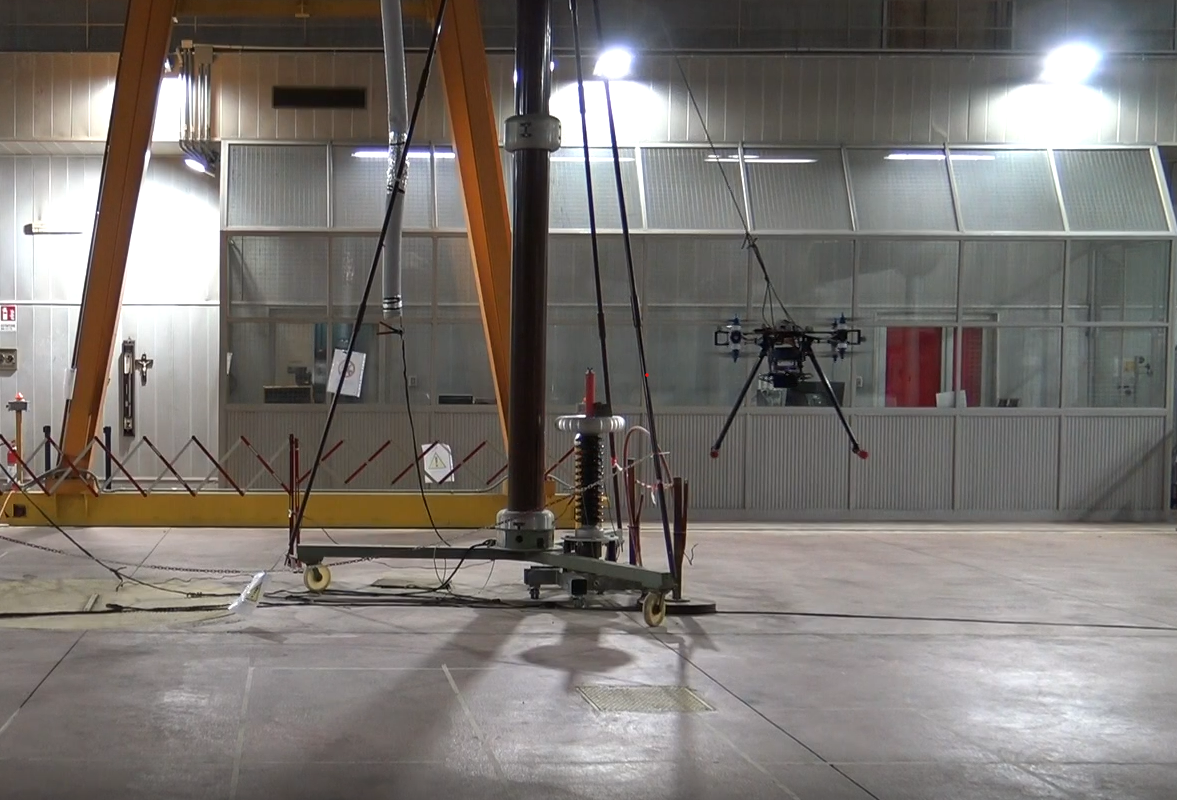
\includegraphics[width=0.75\linewidth]{Immagini/Capitolo7/Experiments/POCHO_flying_arena.png}
    \caption{Snapshot of the physical Observer Drone, \texttt{Pocho}, flying inside the OptiTrack arena during the experimental evaluation.}
    \label{fig:hw_observer_arena}
\end{figure}
The hardware test was intentionally focused on the Observer drone to assess its embedded tracking capabilities, real-time solver execution, and bilateral teleoperation under real aerodynamics, actuator dynamics, and sensor noise. To reduce the computational burden on the onboard companion computer, in these physical experiments jerk and snap penalty terms were omitted from the NMPC cost function. 
Two flight tests were conducted:
\begin{enumerate}
    \item \textbf{Bilateral Haptic Shared Teleoperation Flight:} where the operator actively assigns cylindrical setpoints using the Novint Falcon haptic device, testing online reference tracking, tactile perception, and the APF repulsive forces under human-in-the-loop control.
    \item \textbf{Partial Cooperative Mission Flight:} where the mission FSM commands sequential visual setpoints ($r, \beta, z_{rel}$) across the mission phases while the Observer tracks the moving target, evaluating autonomous viewpoint adaptation and phase progression without executing physical contact with the environment.
\end{enumerate}

\subsection{Bilateral Haptic Shared Teleoperation Flight}
In this first test, the operator interacts with the Novint Falcon haptic device to command time-varying cylindrical setpoints ($r, \beta, z_{rel}$) while the Observer UAV tracks the target quadrotor in real time.

\begin{figure}[htbp]
\centering
\begin{subfigure}[b]{0.71\textwidth}
    
\includegraphics[width=\linewidth]{Immagini/Capitolo7/Experiments/Haptic/phases_legend.pdf}
\end{subfigure}
\begin{subfigure}[b]{0.49\textwidth}
    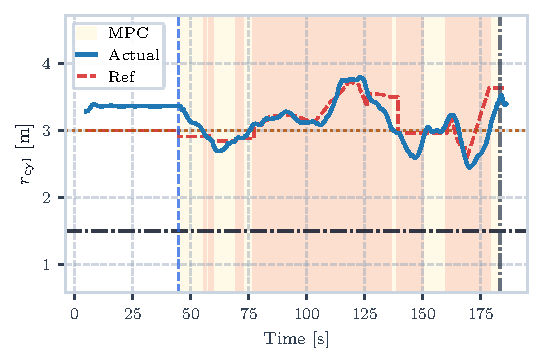
\includegraphics[width=\linewidth]{Immagini/Capitolo7/Experiments/Haptic/CYL_POV_distance_r_cyl.pdf}
\end{subfigure}
\begin{subfigure}[b]{0.49\textwidth}
    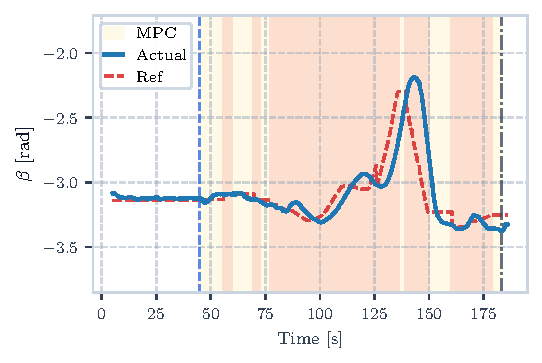
\includegraphics[width=\linewidth]{Immagini/Capitolo7/Experiments/Haptic/CYL_POV_azimuth_beta.pdf}
\end{subfigure}
\begin{subfigure}[b]{0.49\textwidth}
    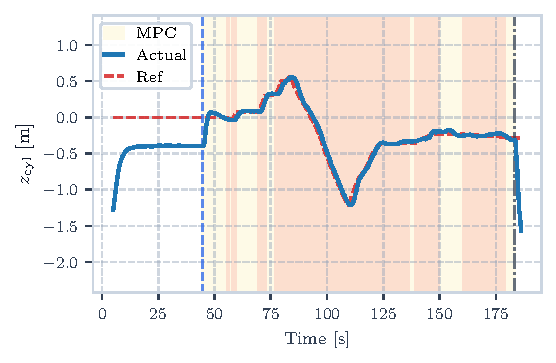
\includegraphics[width=\linewidth]{Immagini/Capitolo7/Experiments/Haptic/CYL_POV_elevation_z.pdf}
\end{subfigure}
\begin{subfigure}[b]{0.49\textwidth}
    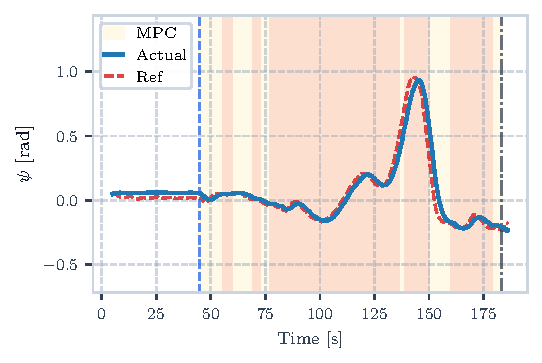
\includegraphics[width=\linewidth]{Immagini/Capitolo7/Experiments/Haptic/YAW_yaw_actual_vs_desired.pdf}
\end{subfigure}
\caption{Cylindrical visual tracking variables during the real-world bilateral haptic teleoperation flight.}
\label{fig:hw_haptic_cyl_pov}
\end{figure}
\justify
Figure~\ref{fig:hw_haptic_cyl_pov} illustrates the tracking performance of the cylindrical coordinates and camera yaw orientation throughout the flight. The colored background bands indicate the active mission phases, during which the human operator continuously commands viewpoint adjustments:
\begin{itemize}
    \item The radial standoff distance $r$ starts from the initial hovering distance ($1.5\text{ m}$) and is actively modified by the operator via the joystick. Despite target velocity variations and real-world disturbances and uncertainties, the observer closely follows the reference, yielding an RMS tracking error of $0.223\text{ m}$ with a maximum deviation of $0.684\text{ m}$.
    \item The azimuth angle $\beta$ shows that the operator successfully commands viewpoint rotations around the target vehicle across different angular sectors. The NMPC navigates the vehicle smoothly along the cylindrical arc, achieving an RMS tracking error of $10.45^\circ$, with a maximum transient peak of $38.94^\circ$ occurring during rapid manual setpoint variations.
    \item The relative elevation $z_{rel}$ demonstrates accurate vertical regulation. The RMS vertical tracking error is limited to $0.062\text{ m}$ ($6.19\text{ cm}$), with a maximum error of $0.398\text{ m}$.
    \item The yaw angle $\psi$ tracks the desired line-of-sight angle computed to point the camera optical axis towards the target drone. The actual yaw closely matches the desired orientation with an RMS error of $4.08^\circ$ (maximum $15.24^\circ$), confirming that the target remains framed in the camera view throughout the teleoperation maneuvers.
\end{itemize}
As shown by the tracking error profiles in Figure~\ref{fig:hw_haptic_cyl_err}, the error norms remain bounded around zero during steady hovering and smooth tracking phases. Error peaks appear only in correspondence with rapid manual setpoint variations or aggressive target maneuvers, after which the NMPC quickly restores visual regulation. In particular, the vertical tracking error $|e_z|$ stays within a few centimeters for almost the entire flight, while the radial distance error $|e_r|$ exhibits higher deviations but without drifting (maximum $60$ cm in correspondence of cumulating references, due to haptic latency), confirming viewpoint maintenance under real aerodynamic disturbances.

\begin{figure}[htbp]
\centering
\begin{subfigure}[b]{0.71\textwidth}
    
\includegraphics[width=\linewidth]{Immagini/Capitolo7/Experiments/Haptic/phases_legend.pdf}
\end{subfigure}
\begin{subfigure}[b]{0.49\textwidth}
    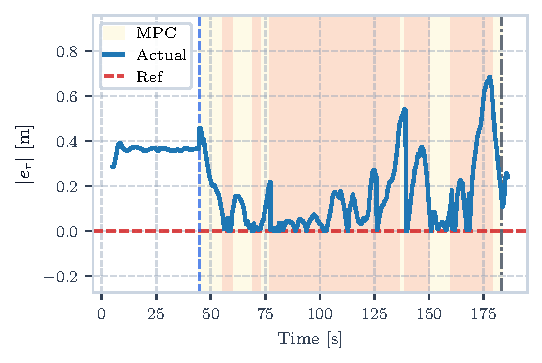
\includegraphics[width=\linewidth]{Immagini/Capitolo7/Experiments/Haptic/CYL_POV_ERR_distance_error_r_cyl_err.pdf}
\end{subfigure}
\begin{subfigure}[b]{0.49\textwidth}
    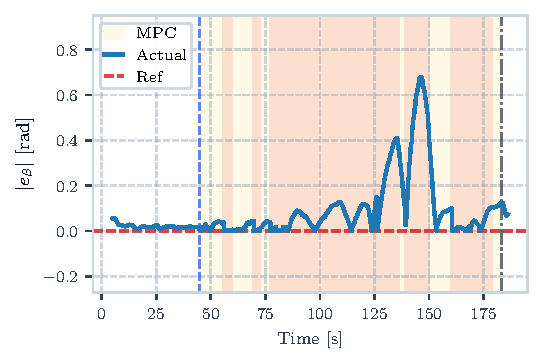
\includegraphics[width=\linewidth]{Immagini/Capitolo7/Experiments/Haptic/CYL_POV_ERR_azimuth_error_beta_err.pdf}
\end{subfigure}
\begin{subfigure}[b]{0.49\textwidth}
    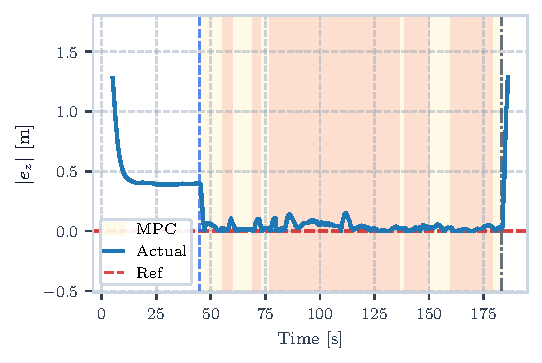
\includegraphics[width=\linewidth]{Immagini/Capitolo7/Experiments/Haptic/CYL_POV_ERR_elevation_error_z_err.pdf}
\end{subfigure}
\begin{subfigure}[b]{0.49\textwidth}
    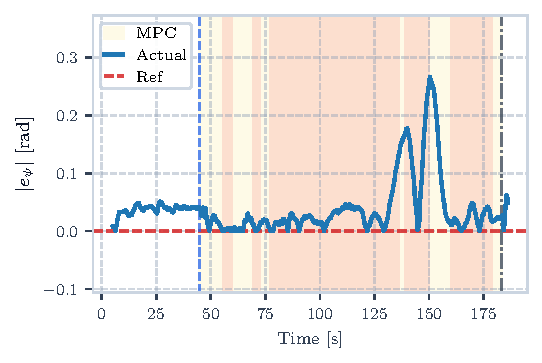
\includegraphics[width=\linewidth]{Immagini/Capitolo7/Experiments/Haptic/CYL_POV_ERR_yaw_error_yaw_err.pdf}
\end{subfigure}
\caption{Tracking error norms on cylindrical coordinates and yaw orientation during the haptic teleoperation flight.}
\label{fig:hw_haptic_cyl_err}
\end{figure}


\begin{figure}[h!]
\centering
\begin{subfigure}[b]{0.51\textwidth}
    
\includegraphics[width=\linewidth]{Immagini/Capitolo7/Experiments/Haptic/phases_legend.pdf}
\end{subfigure}
\begin{subfigure}[b]{0.8\textwidth}
    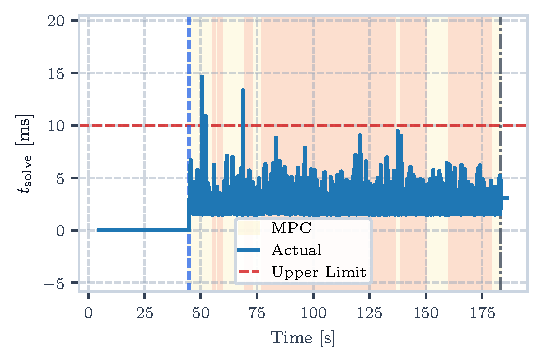
\includegraphics[width=\linewidth]{Immagini/Capitolo7/Experiments/Haptic/SOLVE_TIME_solve_time.pdf}
\end{subfigure}
\caption{Onboard NMPC solving time on the LattePanda companion computer during the haptic teleoperation flight.}
\label{fig:hw_haptic_solve_time}
\end{figure}
\justify
Figure~\ref{fig:hw_haptic_solve_time} reports the execution time of the NMPC solver running onboard the LattePanda companion computer. The mean solve time is $2.29\text{ ms}$, which corresponds to a CPU load of only $22.9\%$ of the available $10\text{ ms}$ sampling period at $100\text{ Hz}$. The 99th percentile of the execution time is $5.88\text{ ms}$, leaving substantial computational headroom for background ROS 2 communications and sensor drivers. Over the entire flight test comprising 3415 consecutive control cycles, only 3 deadline overruns ($>10\text{ ms}$) were detected ($0.09\%$). These isolated delays were quickly absorbed in subsequent cycles without causing any loss of control authority.

\begin{figure}[htbp]
\centering
\begin{subfigure}[b]{0.51\textwidth}
    
\includegraphics[width=\linewidth]{Immagini/Capitolo7/Experiments/Haptic/phases_legend.pdf}
\end{subfigure}
\begin{subfigure}[b]{0.8\textwidth}
    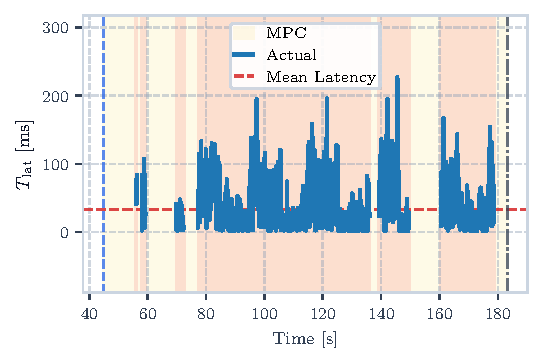
\includegraphics[width=\linewidth]{Immagini/Capitolo7/Experiments/Haptic/HAPTIC_LATENCY_latency.pdf}
\end{subfigure}
\caption{One-way network communication latency of the bilateral haptic teleoperation channel during physical flight.}
\label{fig:hw_haptic_latency}
\end{figure}
\justify
Figure~\ref{fig:hw_haptic_latency} shows the one-way network latency between the Ground Control Station and the onboard companion computer. The communication channel relies on a standard Wi-Fi link transmitting operator setpoints and receiving drone telemetry. The average latency is $32.77\text{ ms}$, with a 95th percentile of $107.04\text{ ms}$. This latency profile proved sufficiently bounded to preserve stability of the bilateral shared-control loop, allowing the operator to perceive force feedback with minimal tactile delay.
\begin{figure}[htbp]
\centering
\begin{subfigure}[b]{0.71\textwidth}
    
\includegraphics[width=\linewidth]{Immagini/Capitolo7/Experiments/Haptic/phases_legend.pdf}
\end{subfigure}
\begin{subfigure}[b]{0.49\textwidth}
    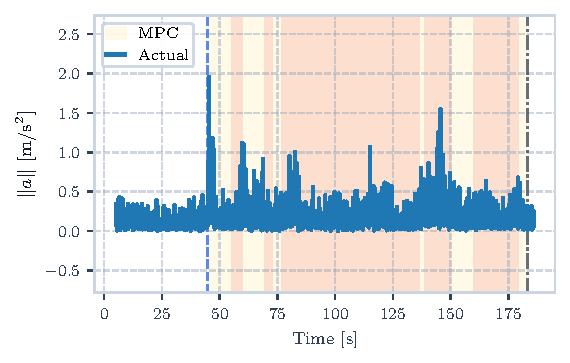
\includegraphics[width=\linewidth]{Immagini/Capitolo7/Experiments/Haptic/DERIVATIVE_NORMS_norm_acc.pdf}
\end{subfigure}
\begin{subfigure}[b]{0.49\textwidth}
    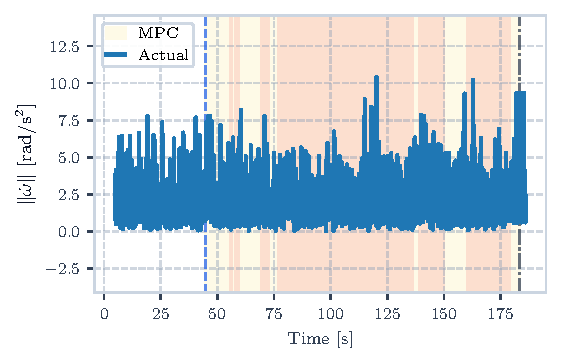
\includegraphics[width=\linewidth]{Immagini/Capitolo7/Experiments/Haptic/DERIVATIVE_NORMS_norm_angacc.pdf}
\end{subfigure}
\begin{subfigure}[b]{0.49\textwidth}
    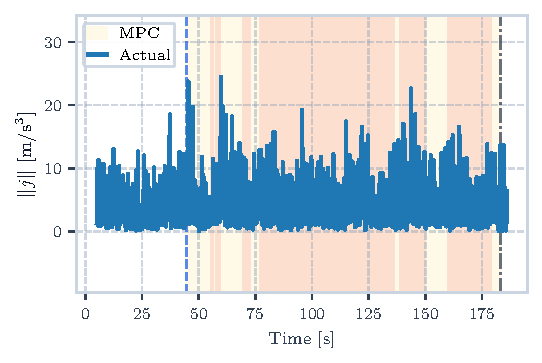
\includegraphics[width=\linewidth]{Immagini/Capitolo7/Experiments/Haptic/DERIVATIVE_NORMS_norm_jerk.pdf}
\end{subfigure}
\begin{subfigure}[b]{0.49\textwidth}
    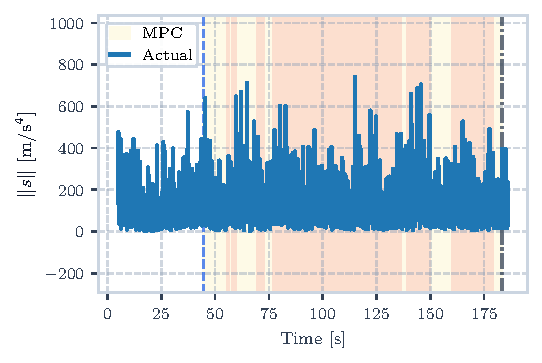
\includegraphics[width=\linewidth]{Immagini/Capitolo7/Experiments/Haptic/DERIVATIVE_NORMS_norm_snap.pdf}
\end{subfigure}
\caption{Norms of higher-order dynamic derivatives recorded during the haptic flight test.}
\label{fig:hw_haptic_derivative_norms}
\end{figure}
\justify
About higher-order time derivatives, figure~\ref{fig:hw_haptic_derivative_norms} presents the norms of linear acceleration $\|a\|$, angular acceleration $\|\dot{\omega}\|$, jerk $\|j\|$, and snap $\|s\|$ recorded during the teleoperation flight. It is worth noting that, in order to keep the solver lightweight on the embedded companion computer, jerk and snap penalty terms were not included in the NMPC cost function during hardware flights. Nevertheless, the physical response remained smooth across all axes: linear acceleration maintained an RMS norm of $0.241\text{ m/s}^2$ (with a peak of $1.95\text{ m/s}^2$ during aggressive maneuvers), and angular velocity had an RMS of $0.099\text{ rad/s}$. The jerk and snap norms show no high-frequency oscillations or chattering, demonstrating that the underlying rigid-body dynamics model and state constraints in the NMPC formulation are sufficient to ensure clean flight behavior.
\\This smooth behavior is also directly reflected in the control wrench, as illustrated in Figure~\ref{fig:hw_haptic_control_wrench}. The vertical thrust $F_z$ stays centered around the nominal hover value ($\approx 37.2\text{ N}$), adapting smoothly to track vertical maneuvers without actuator saturation. The commanded torques remain small and chattering-free; notably, the pitch torque $\tau_y$ shows a consistent steady-state offset around $-0.17\text{ N}\cdot\text{m}$, compensating for the unmodeled forward center-of-mass shift caused by the camera and mounting hardware. The controller easily handles this structural asymmetry, keeping attitude and tracking stable without requiring ad-hoc integrator states.

\begin{figure}[htbp]
\centering
\begin{subfigure}[b]{0.71\textwidth}
    
\includegraphics[width=\linewidth]{Immagini/Capitolo7/Experiments/Haptic/phases_legend.pdf}
\end{subfigure}
\begin{subfigure}[b]{0.49\textwidth}
    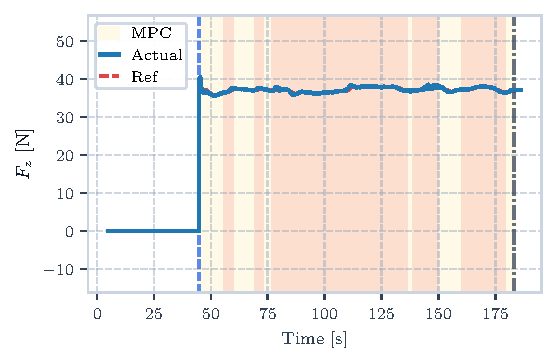
\includegraphics[width=\linewidth]{Immagini/Capitolo7/Experiments/Haptic/CONTROL_WRENCH_force_z.pdf}
\end{subfigure}
\begin{subfigure}[b]{0.49\textwidth}
    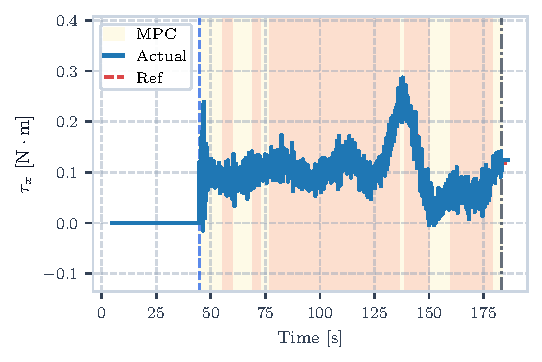
\includegraphics[width=\linewidth]{Immagini/Capitolo7/Experiments/Haptic/CONTROL_WRENCH_torque_x.pdf}
\end{subfigure}
\begin{subfigure}[b]{0.49\textwidth}
    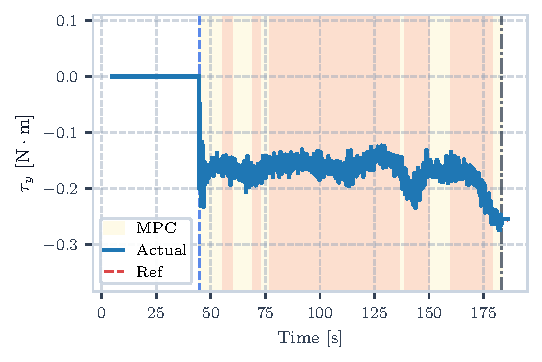
\includegraphics[width=\linewidth]{Immagini/Capitolo7/Experiments/Haptic/CONTROL_WRENCH_torque_y.pdf}
\end{subfigure}
\begin{subfigure}[b]{0.49\textwidth}
    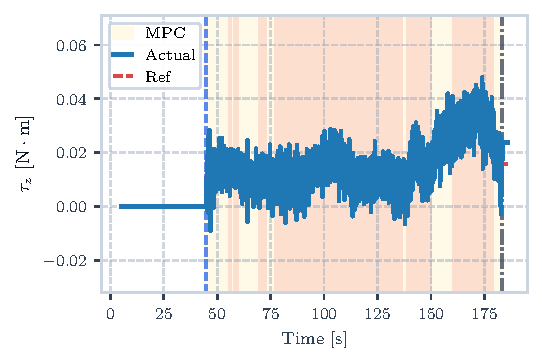
\includegraphics[width=\linewidth]{Immagini/Capitolo7/Experiments/Haptic/CONTROL_WRENCH_torque_z.pdf}
\end{subfigure}
\caption{Control wrench components ($F_z, \tau_x, \tau_y, \tau_z$) commanded by the NMPC during the haptic flight test.}
\label{fig:hw_haptic_control_wrench}
\end{figure}

\begin{figure}[htbp]
\centering
\begin{subfigure}[b]{0.71\textwidth}
    
\includegraphics[width=\linewidth]{Immagini/Capitolo7/Experiments/Haptic/phases_legend.pdf}
\end{subfigure}
\begin{subfigure}[b]{0.32\textwidth}
    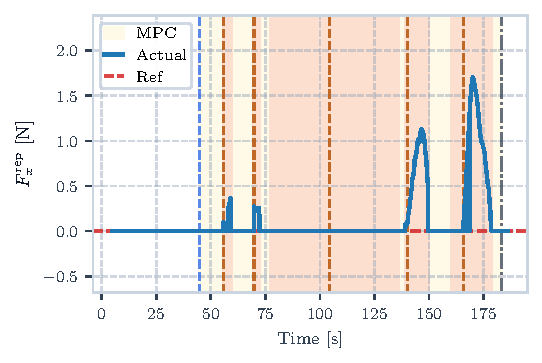
\includegraphics[width=\linewidth]{Immagini/Capitolo7/Experiments/Haptic/REPULSIVE_FORCES_repulsive_force_x.pdf}
\end{subfigure}
\begin{subfigure}[b]{0.32\textwidth}
    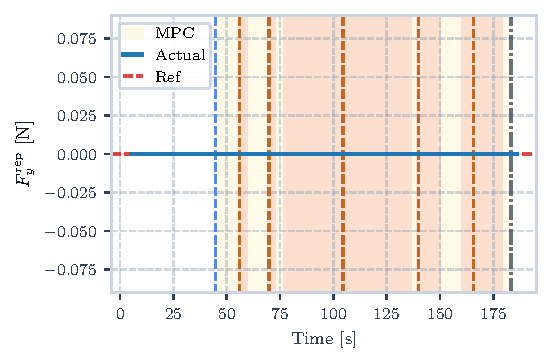
\includegraphics[width=\linewidth]{Immagini/Capitolo7/Experiments/Haptic/REPULSIVE_FORCES_repulsive_force_y.pdf}
\end{subfigure}
\begin{subfigure}[b]{0.32\textwidth}
    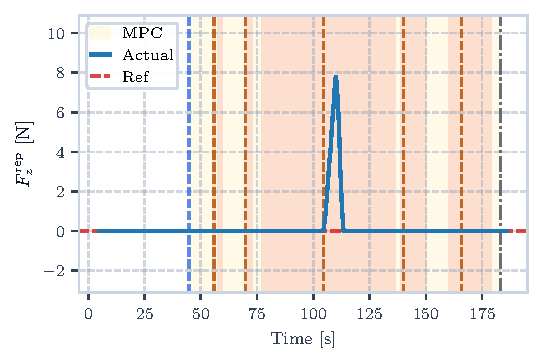
\includegraphics[width=\linewidth]{Immagini/Capitolo7/Experiments/Haptic/REPULSIVE_FORCES_repulsive_force_z.pdf}
\end{subfigure}
\caption{Artificial potential field repulsive forces transmitted to the Novint Falcon joystick during the haptic flight.}
\label{fig:hw_haptic_rep}
\end{figure}

\begin{figure}[htbp]
\centering
\begin{subfigure}[b]{0.71\textwidth}
    
\includegraphics[width=\linewidth]{Immagini/Capitolo7/Experiments/Haptic/phases_legend.pdf}
\end{subfigure}
\begin{subfigure}[b]{0.32\textwidth}
    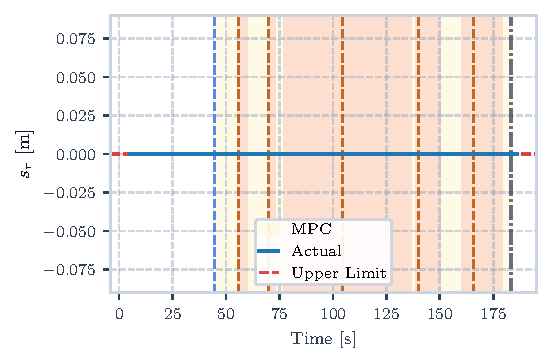
\includegraphics[width=\linewidth]{Immagini/Capitolo7/Experiments/Haptic/APF_distance_violation_s_r.pdf}
\end{subfigure}
\begin{subfigure}[b]{0.32\textwidth}
    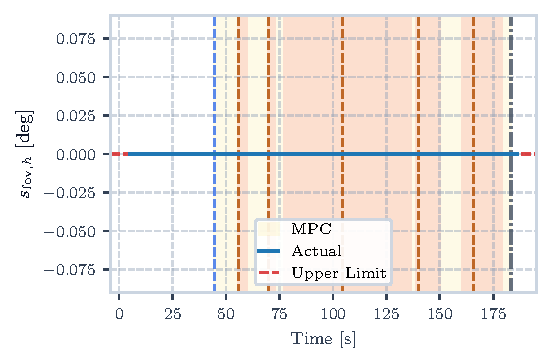
\includegraphics[width=\linewidth]{Immagini/Capitolo7/Experiments/Haptic/APF_horiz_fov_violation_s__fov_h.pdf}
\end{subfigure}
\begin{subfigure}[b]{0.32\textwidth}
    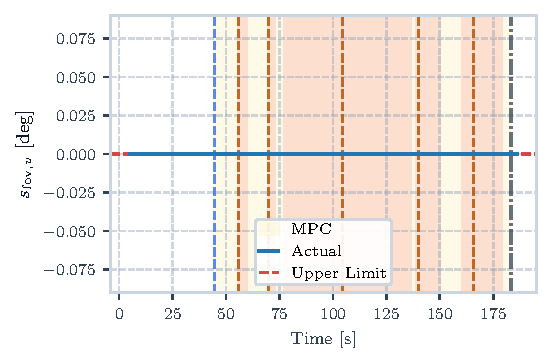
\includegraphics[width=\linewidth]{Immagini/Capitolo7/Experiments/Haptic/APF_vert_fov_violation_s__fov_v.pdf}
\end{subfigure}
\caption{Safety distance and camera Field of View constraint violations during the haptic flight.}
\label{fig:hw_haptic_apf_violations}
\end{figure}
\justify
Figures~\ref{fig:hw_haptic_rep} and \ref{fig:hw_haptic_apf_violations} illustrate the bilateral haptic interaction generated by the Artificial Potential Field (APF). Figure~\ref{fig:hw_haptic_rep} displays the three Cartesian components of the repulsive force ($F_x^{\text{rep}}, F_y^{\text{rep}}, F_z^{\text{rep}}$) sent to the Novint Falcon device, while Figure~\ref{fig:hw_haptic_apf_violations} shows the monitoring of the hard boundary slack variables ($s_r, s_{\text{fov},h}, s_{\text{fov},v}$).
It is worth remarking the relationship between these two figures: as formulated in Section 4.3, the repulsive field does not wait for a hard constraint violation to occur, but activates within an anticipatory buffer zone ($d < d_{\text{act}}$). For the radial distance, the activation threshold is $d_{\text{act}} = 1.5\text{ m}$, meaning tactile resistance begins as soon as $r < 3.0\text{ m}$. In this test, the pilot commanded the drone down to a minimum standoff distance of $2.5\text{ m}$, entering the outer margin of the repulsive zone and receiving a progressive force peaking at $F_x^{\text{rep}} = 1.71\text{ N}$ that discouraged closer approach. Similarly, when commanding vertical viewpoint variations, as the target entered the bottom $30\%$ of the camera frame, the APF rendered an upward repulsive force peaking at $F_z^{\text{rep}} = 7.78\text{ N}$. Guided by this prompt tactile feedback, the operator intuitively adjusted the joystick commands, preventing the vehicle from ever breaching the physical safety distance or losing target line-of-sight. As a result, the boundary violation slacks in Figure~\ref{fig:hw_haptic_apf_violations} remain strictly zero throughout the flight ($s_r = 0.00\text{ m}$, $s_{\text{fov},h} = 0.00^\circ$, $s_{\text{fov},v} = 0.00^\circ$).
\\A comprehensive quantitative summary of the performance metrics for this physical haptic teleoperation flight is reported in Table~\ref{tab:hw_haptic_metrics}.

\begin{table}[htbp]
\centering
\small
\caption{Performance metrics for the real-world bilateral haptic shared teleoperation flight test.}
\label{tab:hw_haptic_metrics}
\begin{tabular}{lc}
\toprule
\textbf{Metric} & \textbf{Value} \\
\midrule
Nominal Control Frequency ($1/T_s$) & \SI{100}{\hertz} \\
Mean Solver Solve Time & \SI{2.29}{\milli\second} (CPU Load: \SI{22.9}{\percent}) \\
99th Percentile Solve Time & \SI{5.88}{\milli\second} \\
Solver Overruns ($> \SI{10}{\milli\second}$) & \SI{0.09}{\percent} ($3 / 3415$) \\
\midrule
Radial Distance RMS / Max Error ($r$) & \SI{0.223}{\meter} / \SI{0.684}{\meter} \\
Azimuth Angle RMS / Max Error ($\beta$) & \ang{10.45} / \ang{38.94} \\
Elevation RMS / Max Error ($z_{rel}$) & \SI{0.062}{\meter} / \SI{0.398}{\meter} \\
Yaw Angle RMS / Max Error ($\psi$) & \ang{4.08} / \ang{15.24} \\
\midrule
Linear Velocity ($\|v\|$) RMS / Max & \SI{0.145}{\meter\per\second} / \SI{0.725}{\meter\per\second} \\
Angular Velocity ($\|\omega\|$) RMS / Max & \SI{0.099}{\radian\per\second} / \SI{0.577}{\radian\per\second} \\
Linear Acceleration ($\|a\|$) RMS / Max & \SI{0.241}{\meter\per\second\squared} / \SI{1.953}{\meter\per\second\squared} \\
\midrule
Max Distance Violation ($s_r$) & \SI{0.000}{\meter} \\
Max Horizontal FoV Violation ($s_{\text{fov},h}$) & \ang{0.00} \\
Max Vertical FoV Violation ($s_{\text{fov},v}$) & \ang{0.00} \\
Max Peak Repulsive Force ($\|F_{\text{rep}}\|_{\infty}$) & \SI{7.78}{\newton} \\
Mean One-Way Haptic Latency & \SI{32.77}{\milli\second} \\
\bottomrule
\end{tabular}
\end{table}

\subsection{Partial Mission Flight Test}
The second physical experiment evaluates the autonomous execution of a partial cooperative mission. In this test, the mission Finite State Machine orchestrates the sequential phases (Takeoff, Approach, Interaction, Detachment, Landing), updating the nominal cylindrical setpoints $(r, \beta, z_{rel})$ at each phase transition. The target quadrotor was flown manually inside the arena to provide an active, moving target, while the Observer UAV executed autonomous trajectory tracking and viewpoint reconfiguration without performing physical contact with the environment.

\begin{figure}[htbp]
\centering
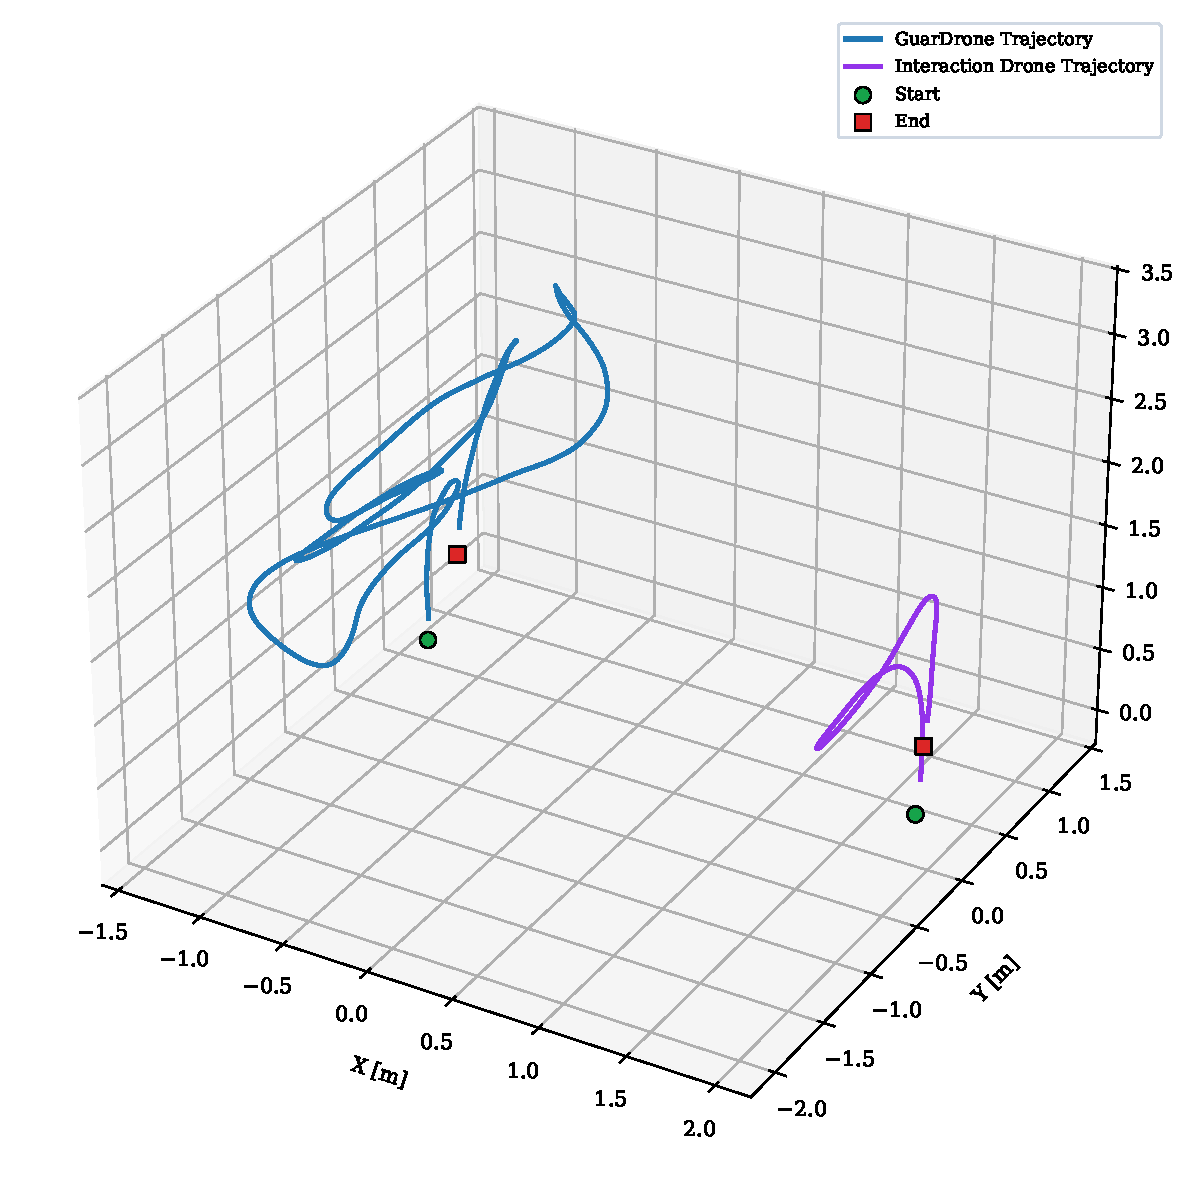
\includegraphics[width=0.55\linewidth]{Immagini/Capitolo7/Experiments/Mission/3D.pdf}
\caption{3D trajectories of the Observer and Target UAVs during the partial mission flight test.}
\label{fig:hw_mission_3d}
\end{figure}
\justify
Figure~\ref{fig:hw_mission_3d} shows the spatial trajectories of both vehicles reconstructed from OptiTrack telemetry. The Observer UAV continuously tracks the target across the three-dimensional volume, maintaining the commanded standoff distance and circling around it to achieve the perspective required by each operational phase.

\begin{figure}[htbp]
\centering
\begin{subfigure}[b]{0.71\textwidth}
    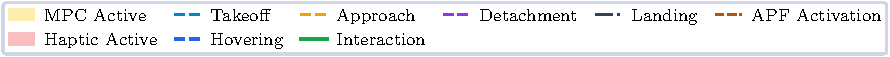
\includegraphics[width=\linewidth]{Immagini/Capitolo7/Experiments/Mission/phases_legend.pdf}
\end{subfigure}
\begin{subfigure}[b]{0.49\textwidth}
    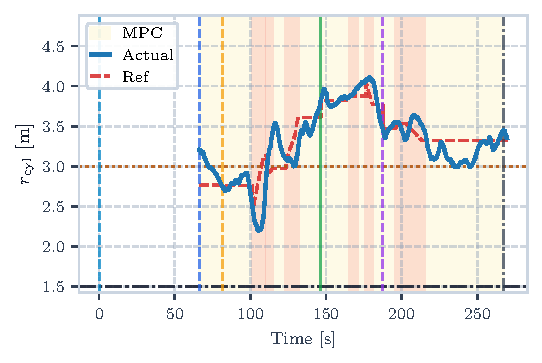
\includegraphics[width=\linewidth]{Immagini/Capitolo7/Experiments/Mission/CYL_POV_distance_r_cyl.pdf}
\end{subfigure}
\begin{subfigure}[b]{0.49\textwidth}
    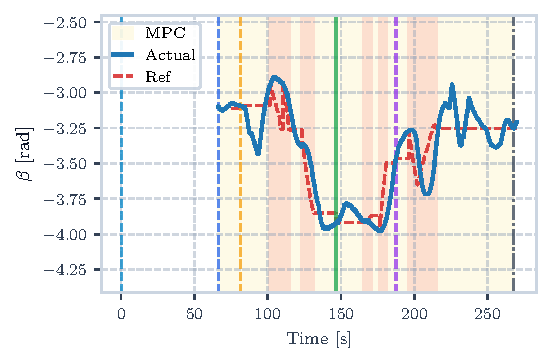
\includegraphics[width=\linewidth]{Immagini/Capitolo7/Experiments/Mission/CYL_POV_azimuth_beta.pdf}
\end{subfigure}
\begin{subfigure}[b]{0.49\textwidth}
    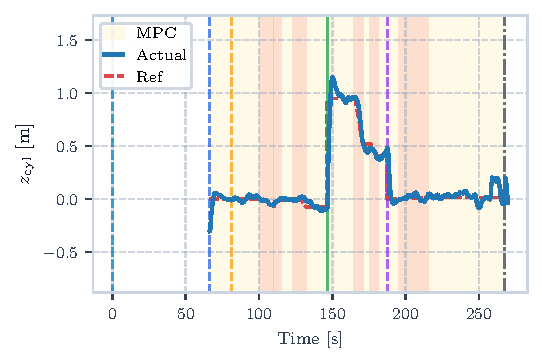
\includegraphics[width=\linewidth]{Immagini/Capitolo7/Experiments/Mission/CYL_POV_elevation_z.pdf}
\end{subfigure}
\begin{subfigure}[b]{0.49\textwidth}
    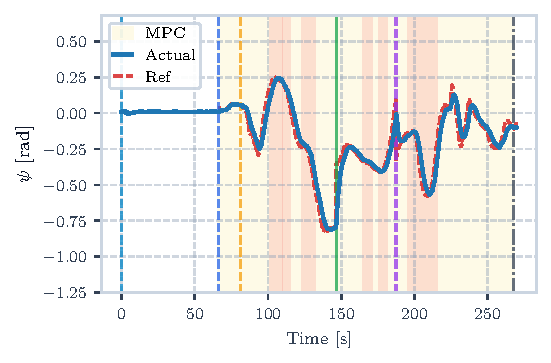
\includegraphics[width=\linewidth]{Immagini/Capitolo7/Experiments/Mission/YAW_yaw_actual_vs_desired.pdf}
\end{subfigure}
\caption{Cylindrical visual tracking variables during the real-world partial mission flight test.}
\label{fig:hw_mission_cyl_pov}
\end{figure}
\justify
Figure~\ref{fig:hw_mission_cyl_pov} details the tracking of the relative cylindrical coordinates across the mission phases:
\begin{itemize}
    \item The radial distance $r$ transitions from takeoff to the nominal standoff distance ($1.5\text{ m}$) and follows the phase references with an RMS error of $0.214\text{ m}$ (max $0.768\text{ m}$).
    \item The azimuth angle $\beta$ tracks the discrete step changes commanded by the supervisor between consecutive mission phases, demonstrating smooth convergence to the new perspective with an RMS error of $8.58^\circ$ (maximum transient deviation of $23.07^\circ$).
    \item The relative elevation $z_{rel}$ adapts to the nominal altitude offsets prescribed by the FSM, achieving an RMS tracking error of $0.082\text{ m}$ ($8.20\text{ cm}$) with a maximum error of $1.040\text{ m}$.
    \item The yaw orientation $\psi$ continuously aligns with the target heading reference, maintaining an RMS tracking error of $3.98^\circ$ (maximum $25.30^\circ$).
\end{itemize}
These results confirm that the NMPC tracker smoothly absorbs discrete phase step references, preserving trajectory continuity without inducing overshoot or flight instability.

The tracking errors on the cylindrical variables are shown in Figure~\ref{fig:hw_mission_cyl_err}. In this test, each phase transition commanded by the FSM introduces a discrete step in the reference (such as the viewpoint shift entering the Interaction phase). As it is visible from the plots, these steps produce temporary transient errors that the NMPC promptly rejects within a few seconds, driving the errors back to zero. Even under the continuous manual motion of the target vehicle, the radial distance error $|e_r|$ maintains an RMS of $0.214\text{ m}$ and the azimuth error $|e_\beta|$ stays at $8.58^\circ$, demonstrating effective viewpoint synchronization across all phases.

\begin{figure}[htbp]
\centering
\begin{subfigure}[b]{0.71\textwidth}
    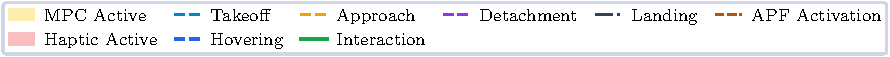
\includegraphics[width=\linewidth]{Immagini/Capitolo7/Experiments/Mission/phases_legend.pdf}
\end{subfigure}
\begin{subfigure}[b]{0.49\textwidth}
    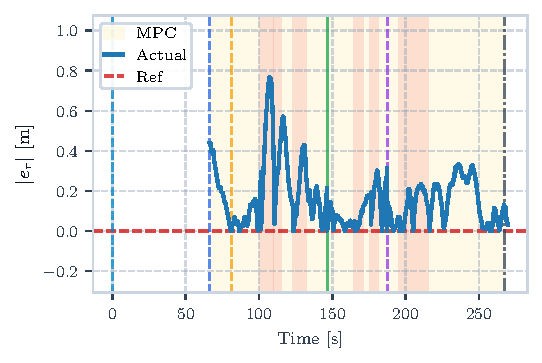
\includegraphics[width=\linewidth]{Immagini/Capitolo7/Experiments/Mission/CYL_POV_ERR_distance_error_r_cyl_err.pdf}
\end{subfigure}
\begin{subfigure}[b]{0.49\textwidth}
    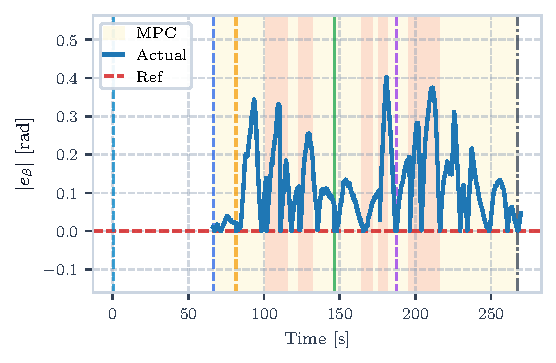
\includegraphics[width=\linewidth]{Immagini/Capitolo7/Experiments/Mission/CYL_POV_ERR_azimuth_error_beta_err.pdf}
\end{subfigure}
\begin{subfigure}[b]{0.49\textwidth}
    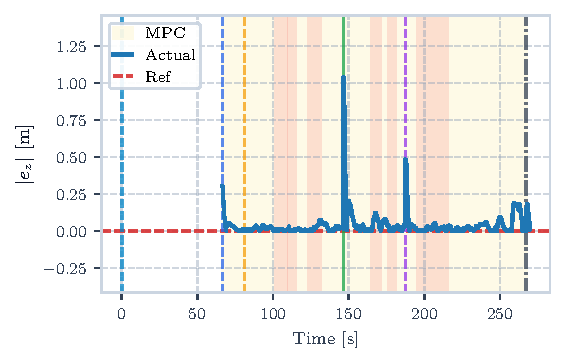
\includegraphics[width=\linewidth]{Immagini/Capitolo7/Experiments/Mission/CYL_POV_ERR_elevation_error_z_err.pdf}
\end{subfigure}
\begin{subfigure}[b]{0.49\textwidth}
    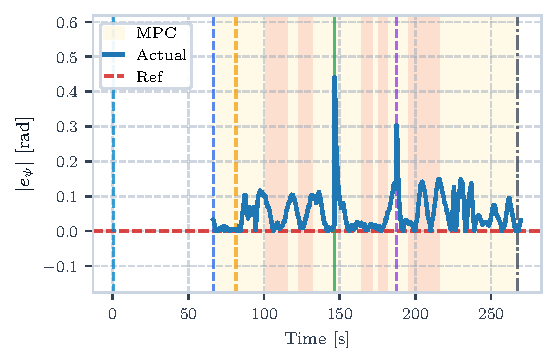
\includegraphics[width=\linewidth]{Immagini/Capitolo7/Experiments/Mission/CYL_POV_ERR_yaw_error_yaw_err.pdf}
\end{subfigure}
\caption{Tracking error norms on cylindrical coordinates and yaw orientation during the mission flight test.}
\label{fig:hw_mission_cyl_err}
\end{figure}


\begin{figure}[htbp]
\centering
\begin{subfigure}[b]{0.49\textwidth}
    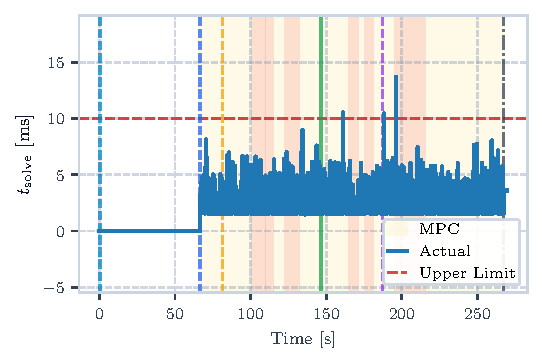
\includegraphics[width=\linewidth]{Immagini/Capitolo7/Experiments/Mission/SOLVE_TIME_solve_time.pdf}
    \caption{Onboard NMPC solving time}
    \label{fig:hw_mission_solve_time}
\end{subfigure}
\hfill
\begin{subfigure}[b]{0.49\textwidth}
    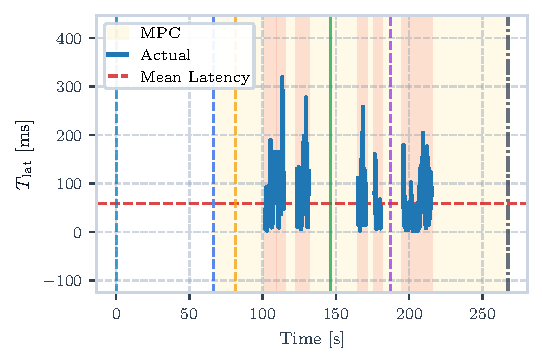
\includegraphics[width=\linewidth]{Immagini/Capitolo7/Experiments/Mission/HAPTIC_LATENCY_latency.pdf}
    \caption{Network communication latency}
    \label{fig:hw_mission_latency}
\end{subfigure}
\caption{Computational timing and communication latency during the real-world partial mission flight test.}
\label{fig:hw_mission_timing}
\end{figure}
\justify
Figure~\ref{fig:hw_mission_timing} displays the real-time execution statistics for the mission flight test. 
Specifically, Figure~\ref{fig:hw_mission_solve_time} shows the onboard NMPC solver execution time on the companion computer. The mean solve time is $2.29\text{ ms}$, corresponding to $22.9\%$ CPU load at $100\text{ Hz}$, with a 99th percentile of $6.02\text{ ms}$. Over 4762 consecutive execution cycles, only 3 deadline overruns occurred ($0.06\%$), demonstrating consistent real-time determinism throughout the entire mission duration.
Figure~\ref{fig:hw_mission_latency} reports the one-way network communication latency between the GCS and the onboard system, which averaged $59.28\text{ ms}$. Despite typical wireless jitter, telemetry and commands remained continuously synchronized without packet loss.

\begin{figure}[htbp]
\centering
\begin{subfigure}[b]{0.71\textwidth}
    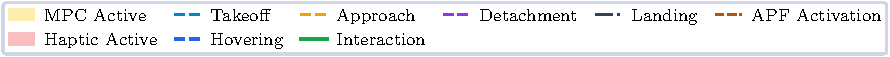
\includegraphics[width=\linewidth]{Immagini/Capitolo7/Experiments/Mission/phases_legend.pdf}
\end{subfigure}
\begin{subfigure}[b]{0.49\textwidth}
    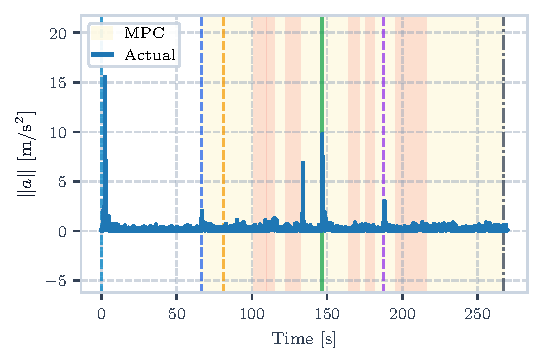
\includegraphics[width=\linewidth]{Immagini/Capitolo7/Experiments/Mission/DERIVATIVE_NORMS_norm_acc.pdf}
\end{subfigure}
\begin{subfigure}[b]{0.49\textwidth}
    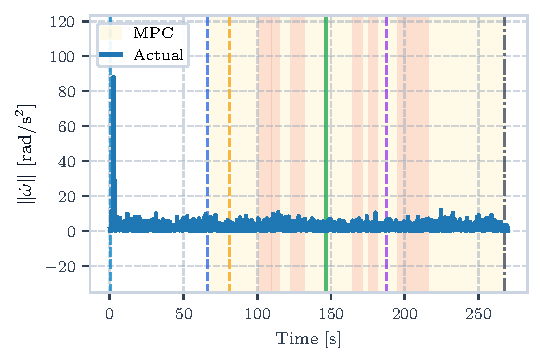
\includegraphics[width=\linewidth]{Immagini/Capitolo7/Experiments/Mission/DERIVATIVE_NORMS_norm_angacc.pdf}
\end{subfigure}
\begin{subfigure}[b]{0.49\textwidth}
    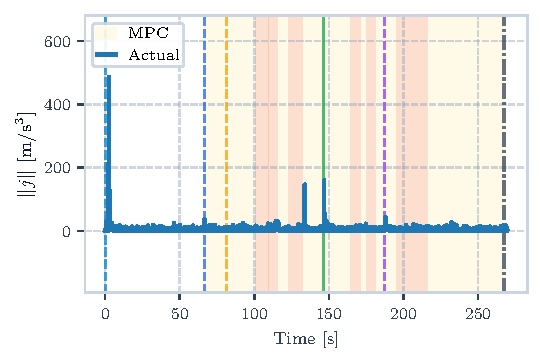
\includegraphics[width=\linewidth]{Immagini/Capitolo7/Experiments/Mission/DERIVATIVE_NORMS_norm_jerk.pdf}
\end{subfigure}
\begin{subfigure}[b]{0.49\textwidth}
    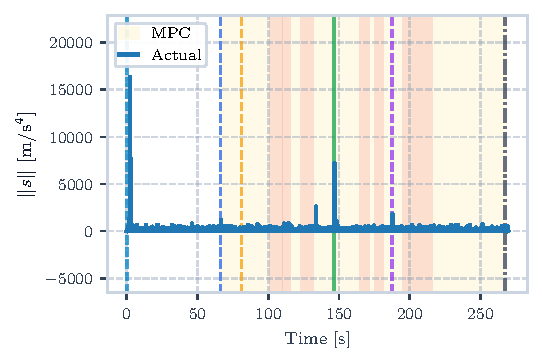
\includegraphics[width=\linewidth]{Immagini/Capitolo7/Experiments/Mission/DERIVATIVE_NORMS_norm_snap.pdf}
\end{subfigure}
\caption{Norms of higher-order dynamic derivatives recorded during the partial mission flight.}
\label{fig:hw_mission_derivative_norms}
\end{figure}
\justify
Figure~\ref{fig:hw_mission_derivative_norms} presents the dynamic derivative norms recorded during the mission flight. As in the teleoperation test, jerk and snap penalty terms were excluded from the cost function to preserve onboard computational resources. Even without explicit higher-order regularization, linear velocity remained strictly contained ($0.137\text{ m/s}$ RMS, $0.815\text{ m/s}$ maximum), and linear acceleration exhibited an RMS norm of $0.495\text{ m/s}^2$ ($15.533\text{ m/s}^2$ peak during abrupt phase step commands). The vehicle navigated between viewpoints without excessive oscillations.
Furthermore, no distance or camera FoV constraint violations occurred throughout the test ($s_r = 0.00\text{ m}$, $s_{\text{fov},h} = 0.00^\circ$, $s_{\text{fov},v} = 0.00^\circ$), with the APF generating a maximum peak repulsive force of $3.04\text{ N}$.

Looking at the control wrench components reported in Figure~\ref{fig:hw_mission_control_wrench}, the generated control actions remain smooth and well within the feasible actuation envelope throughout the flight. The total thrust $F_z$ averages $38.06\text{ N}$, with moderate variations during altitude reconfigurations and no saturation. In agreement with the previous test, the torque components are devoid of chattering, and $\tau_y$ continuously counterbalances the front camera pitch torque with a steady mean of $-0.18\text{ N}\cdot\text{m}$, further validating the real-world stability and robustness of the control outputs.

\begin{figure}[htbp]
\centering
\begin{subfigure}[b]{0.71\textwidth}
    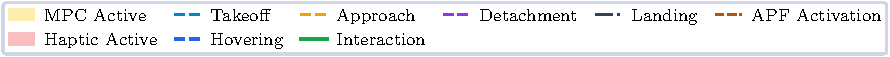
\includegraphics[width=\linewidth]{Immagini/Capitolo7/Experiments/Mission/phases_legend.pdf}
\end{subfigure}
\begin{subfigure}[b]{0.49\textwidth}
    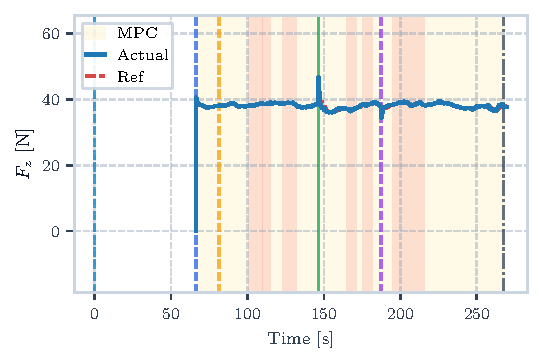
\includegraphics[width=\linewidth]{Immagini/Capitolo7/Experiments/Mission/CONTROL_WRENCH_force_z.pdf}
\end{subfigure}
\begin{subfigure}[b]{0.49\textwidth}
    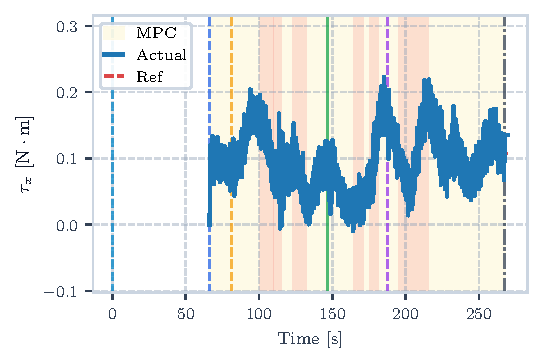
\includegraphics[width=\linewidth]{Immagini/Capitolo7/Experiments/Mission/CONTROL_WRENCH_torque_x.pdf}
\end{subfigure}
\begin{subfigure}[b]{0.49\textwidth}
    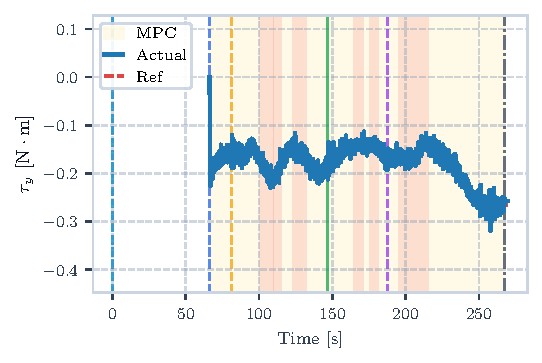
\includegraphics[width=\linewidth]{Immagini/Capitolo7/Experiments/Mission/CONTROL_WRENCH_torque_y.pdf}
\end{subfigure}
\begin{subfigure}[b]{0.49\textwidth}
    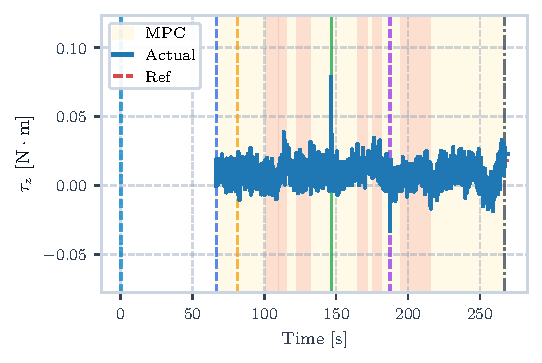
\includegraphics[width=\linewidth]{Immagini/Capitolo7/Experiments/Mission/CONTROL_WRENCH_torque_z.pdf}
\end{subfigure}
\caption{Control wrench components ($F_z, \tau_x, \tau_y, \tau_z$) commanded by the NMPC during the partial mission flight test.}
\label{fig:hw_mission_control_wrench}
\end{figure}
The complete set of performance metrics for the mission flight test is summarized in Table~\ref{tab:hw_mission_metrics}.
\begin{table}[htbp]
\centering
\small
\caption{Performance metrics and benchmark for the real-world partial cooperative mission flight test.}
\label{tab:hw_mission_metrics}
\begin{tabular}{lc}
\toprule
\textbf{Metric} & \textbf{Value} \\
\midrule
Nominal Control Frequency ($1/T_s$) & \SI{100}{\hertz} \\
Mean Solver Solve Time & \SI{2.29}{\milli\second} (CPU Load: \SI{22.9}{\percent}) \\
99th Percentile Solve Time & \SI{6.02}{\milli\second} \\
Solver Overruns ($> \SI{10}{\milli\second}$) & \SI{0.06}{\percent} ($3 / 4762$) \\
\midrule
Radial Distance RMS / Max Error ($r$) & \SI{0.214}{\meter} / \SI{0.768}{\meter} \\
Azimuth Angle RMS / Max Error ($\beta$) & \ang{8.58} / \ang{23.07} \\
Elevation RMS / Max Error ($z_{rel}$) & \SI{0.082}{\meter} / \SI{1.040}{\meter} \\
Yaw Angle RMS / Max Error ($\psi$) & \ang{3.98} / \ang{25.30} \\
\midrule
Linear Velocity ($\|v\|$) RMS / Max & \SI{0.137}{\meter\per\second} / \SI{0.815}{\meter\per\second} \\
Angular Velocity ($\|\omega\|$) RMS / Max & \SI{0.113}{\radian\per\second} / \SI{1.688}{\radian\per\second} \\
Linear Acceleration ($\|a\|$) RMS / Max & \SI{0.495}{\meter\per\second\squared} / \SI{15.533}{\meter\per\second\squared} \\
\midrule
Max Distance Violation ($s_r$) & \SI{0.000}{\meter} \\
Max Horizontal FoV Violation ($s_{\text{fov},h}$) & \ang{0.00} \\
Max Vertical FoV Violation ($s_{\text{fov},v}$) & \ang{0.00} \\
Max Peak Repulsive Force ($\|F_{\text{rep}}\|_{\infty}$) & \SI{3.04}{\newton} \\
Mean One-Way Haptic Latency & \SI{59.28}{\milli\second} \\
\bottomrule
\end{tabular}
\end{table}

These experimental flight tests successfully demonstrate the feasibility and robustness of the embedded NMPC formulation and bilateral haptic teleoperation on real multirotor hardware under actual sensor noise, aerodynamic disturbances, and wireless communication latencies.